\documentclass[a4paper]{article}

\usepackage[english]{babel}
\usepackage[utf8x]{inputenc}
\usepackage{amsmath}
\usepackage{amsfonts}
\usepackage{graphicx}
\usepackage{subfigure}
\usepackage{url}
\usepackage[colorinlistoftodos]{todonotes}

\title{CS 5785 -- Applied Machine Learning -- Lec.\ 5}
\author{Prof.\ Nathan Kallus, Cornell Tech\\Scribes: Ben Hwang, Ben Yellin, Haojie Zhang, \\Kulvinder Lotay, Omer Winarunke, Shantanu Phadke}
\date{September 6, 2017}

\begin{document}
\maketitle

\section{Recap - Logistic Regression}
\subsection{Logit / Log Odds Function}
The Logit or Log Odds function is a mapping from the probability values in range $[0,1]$ to $(\infty, -\infty)$. It is also the inverse of the sigmoid function, which maps values in the range $(\infty, -\infty)$ to probabilities in the range $[0, 1]$. The logit function is as follows:

\begin{equation}
    \text{logit(p)} = \log\Big(\frac{p}{1-p}\Big)
\end{equation}
The following is a graph of the logit function:
\begin{center}
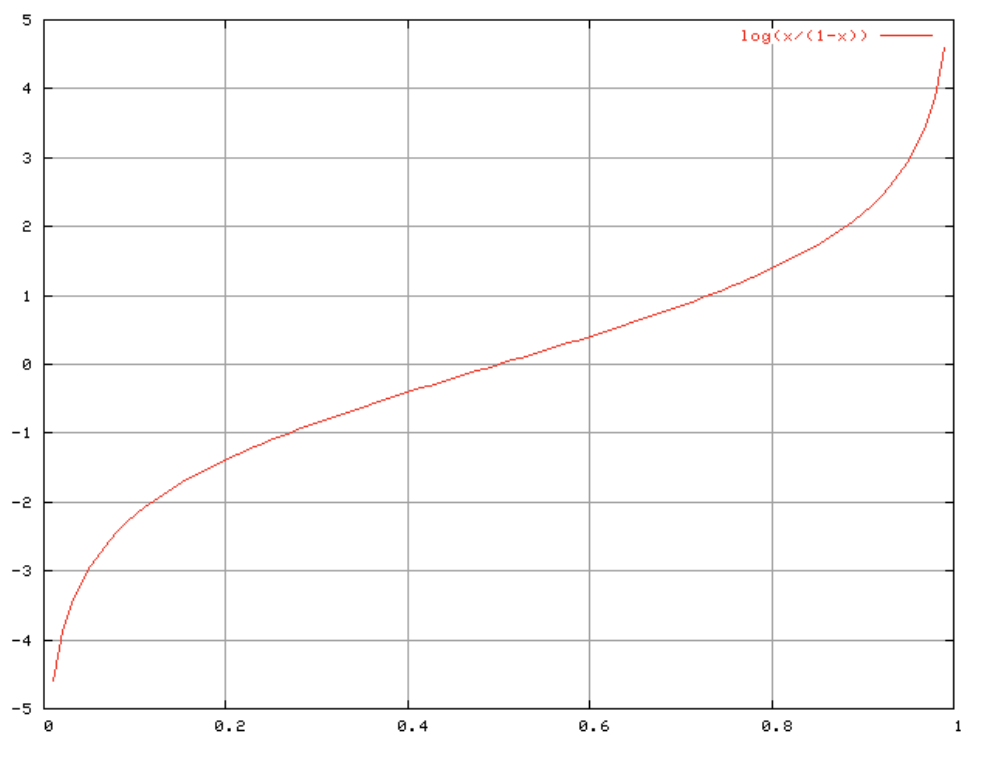
\includegraphics[width=300px, height=180px]{logit_function.png}
\end{center}

The inverse of the logit function is as follows:

\begin{equation}
    \text{logit}^{-1}\text{(p)} = \frac{1}{1+\text{exp}(-\alpha)} = \frac{\text{exp}(\alpha)}{1+\text{exp}(\alpha)}
\end{equation}
\subsection{Standard Logistic Sigmoid Function}
The Standard Logistic Sigmoid Function maps values in the range $(-\infty, \infty)$  to probabilities in the range $[0, 1]$. The function is as follows:
\begin{equation}
    \text{P(t)} = \frac{1}{1 + e^{-t}}
\end{equation}
Additionally it is good to know some key properties of the sigmoid function:
\begin{equation}
    \frac{\text{d}}{\text{dt}}\text{P(t)} = \text{P(t)}\times (1-\text{P(t)})
\end{equation}
\begin{equation}
    1 - \text{P(t)} = \text{P(-t)}
\end{equation}
Additionally, the graph of the sigmoid function looks like the following:
\begin{center}
    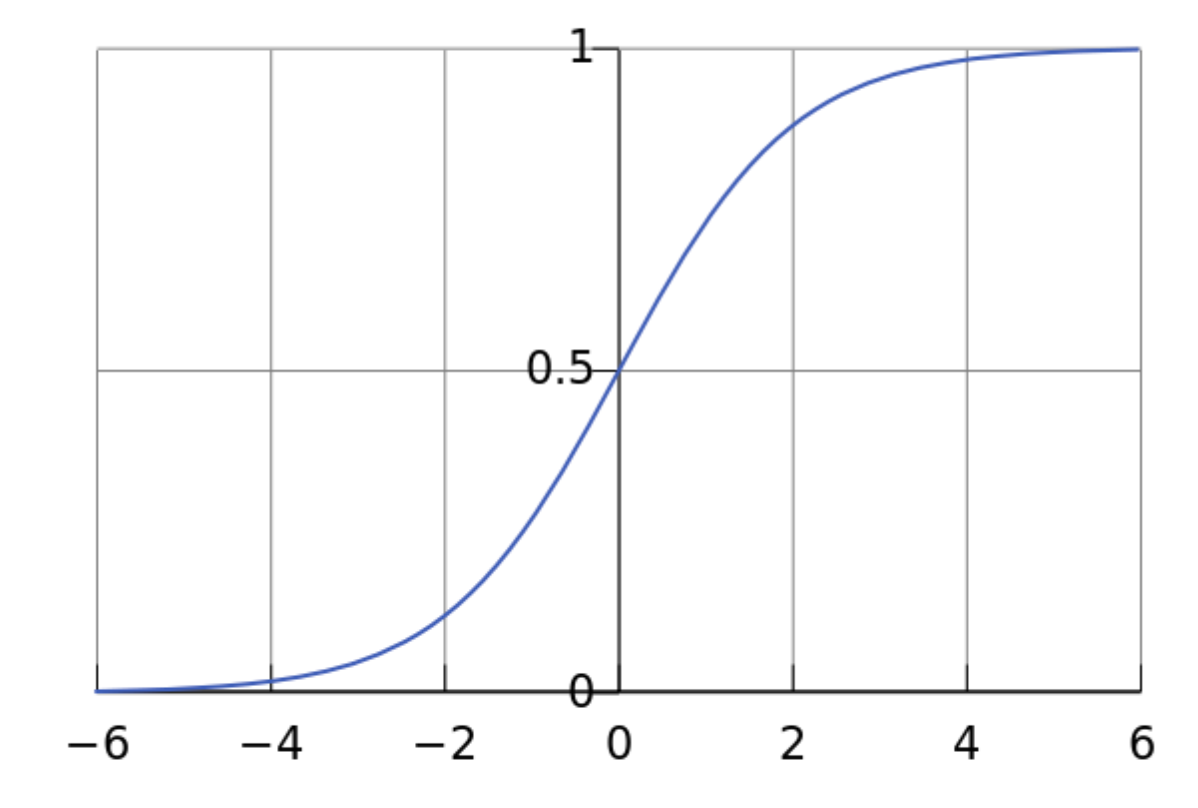
\includegraphics[width=300px, height=180px]{sigmoid_function.png}
\end{center}
\subsection{Linear Model vs Logistic Model}
Where as in the Linear Regression model we are trying to find a line in the form $y = b_{0} + b_{1}x$ that best fits our given data, in the case of Logistic Regression models we are trying to best fit the function $p = \frac{1}{1 + e^{-(b_{0}+b_{1}x)}}$ to our given data.\\\\
There are some fundamental differences for when we would use Linear Regression models and Logistic Regression models. The main difference is that Linear Regression models are meant for data that is continuous in nature, where as Logistic Regression models are more fit for Binary Classification problems where we need to predict which of two classes given data points belong to.\\\\
The following graph displays the visual difference between these two types of models:
\begin{center}
    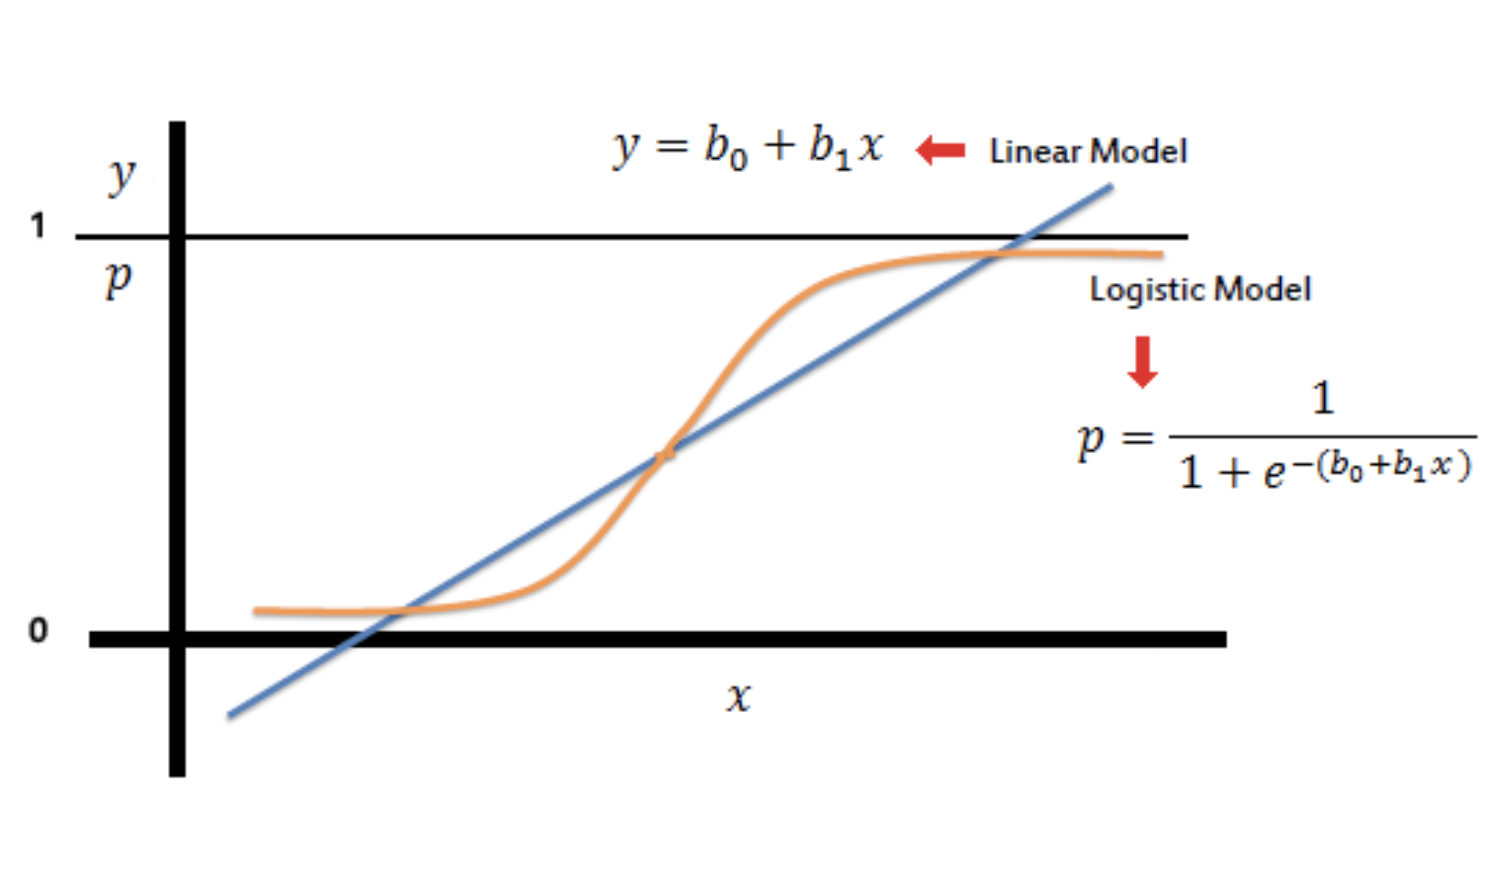
\includegraphics[width=300px, height=180px]{linear_vs_logistic.png}
\end{center}
In this sense the Logistic Regression model above assigns a probability to each of the points (represented by p), where p is the probability that the specific point has a label of 1. Thus, the higher p is the closer the function is to y=1, and the lower p is the closer it is to y=0.

\subsection{Logistic Regression Example: Hours Spent Studying vs Passing Exam}
An example of a situation in which we can apply a Logistic Regression model is a scenario where we are coming up a system to predict the probability of a student passing a test given the number of hours they have studied as input. This data is ideal for a Logistic Regression model for two main reasons:\\\\
\indent(a) The input data points will be in the form (x,y) where x will be the number of hours a particu \indent lar student studied for the exam in question, and y is an integer in the set $\{0,1\}$ where 0 represents that \indent the student didn't pass the exam, and 1 represents that the student has passed the exam.\\\\
\indent(b) Since we can't get a model that exactly models this scenario correctly 100\% of the time, we es \indent timate it via forming a probability distribution by utilizing the Logistic Regression function.\\\\
Let's say our original data set looks as follows when plotted out:
\begin{center}
    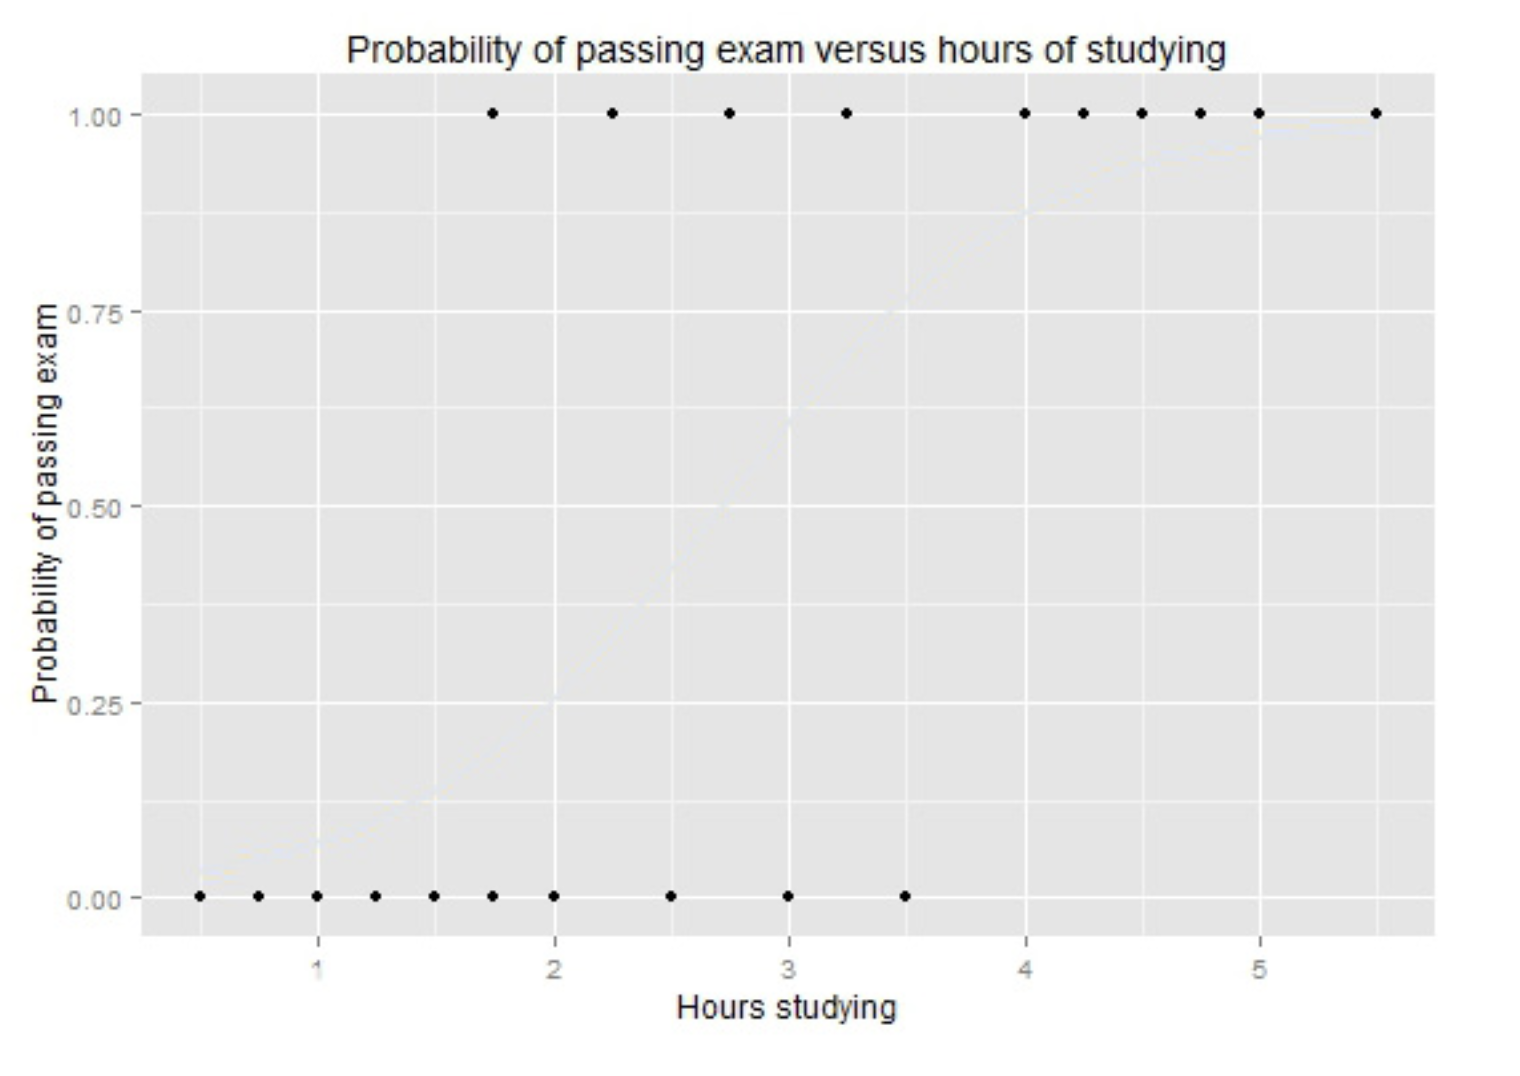
\includegraphics[width=300px, height=180px]{sample_dataset.png}
\end{center}
Then our Logistic Regression Model to estimate the probability that each student would pass the exam given the number of hours they have studied overlaid on this data would look as follows:
\begin{center}
    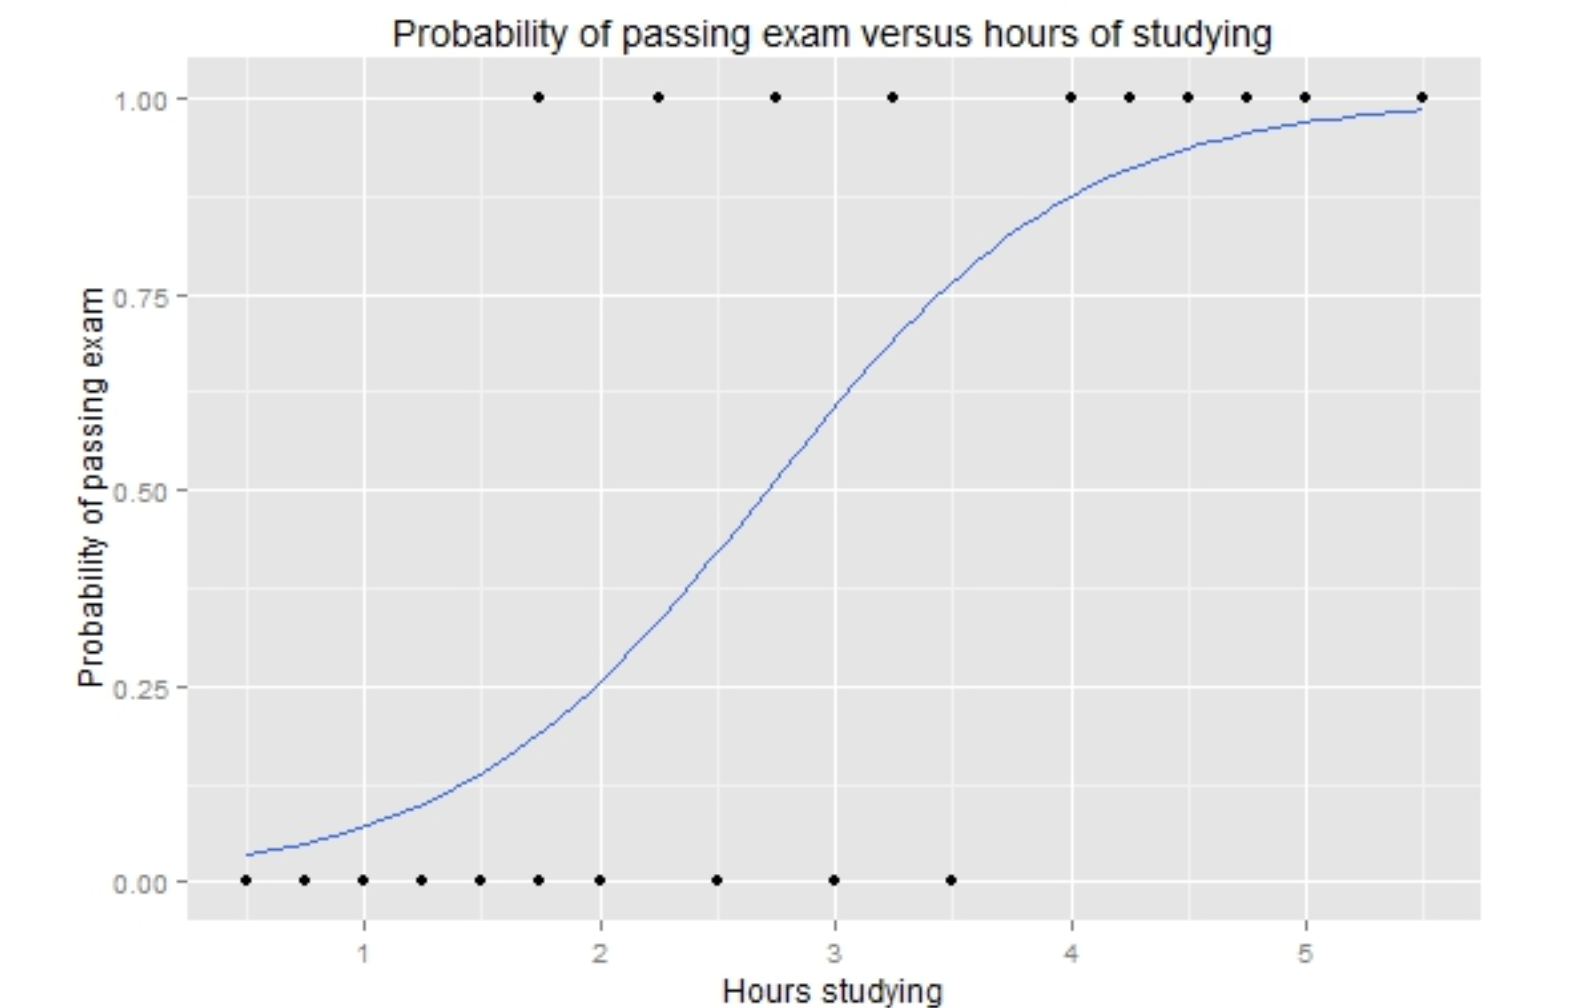
\includegraphics[width=300px,height=180px]{overlay.png}
\end{center}
\subsection{Advantage of Logistic Regression over Linear Regression}
Besides the usage case difference between the two, another big advantage Logistic Regression has over Linear Regression is that the decision boundary produced by Logistic Regression is significantly less sensitive to outliers than Decision Boundaries produced by Linear Regression models, as illustrated by the figure below:
\begin{center}
    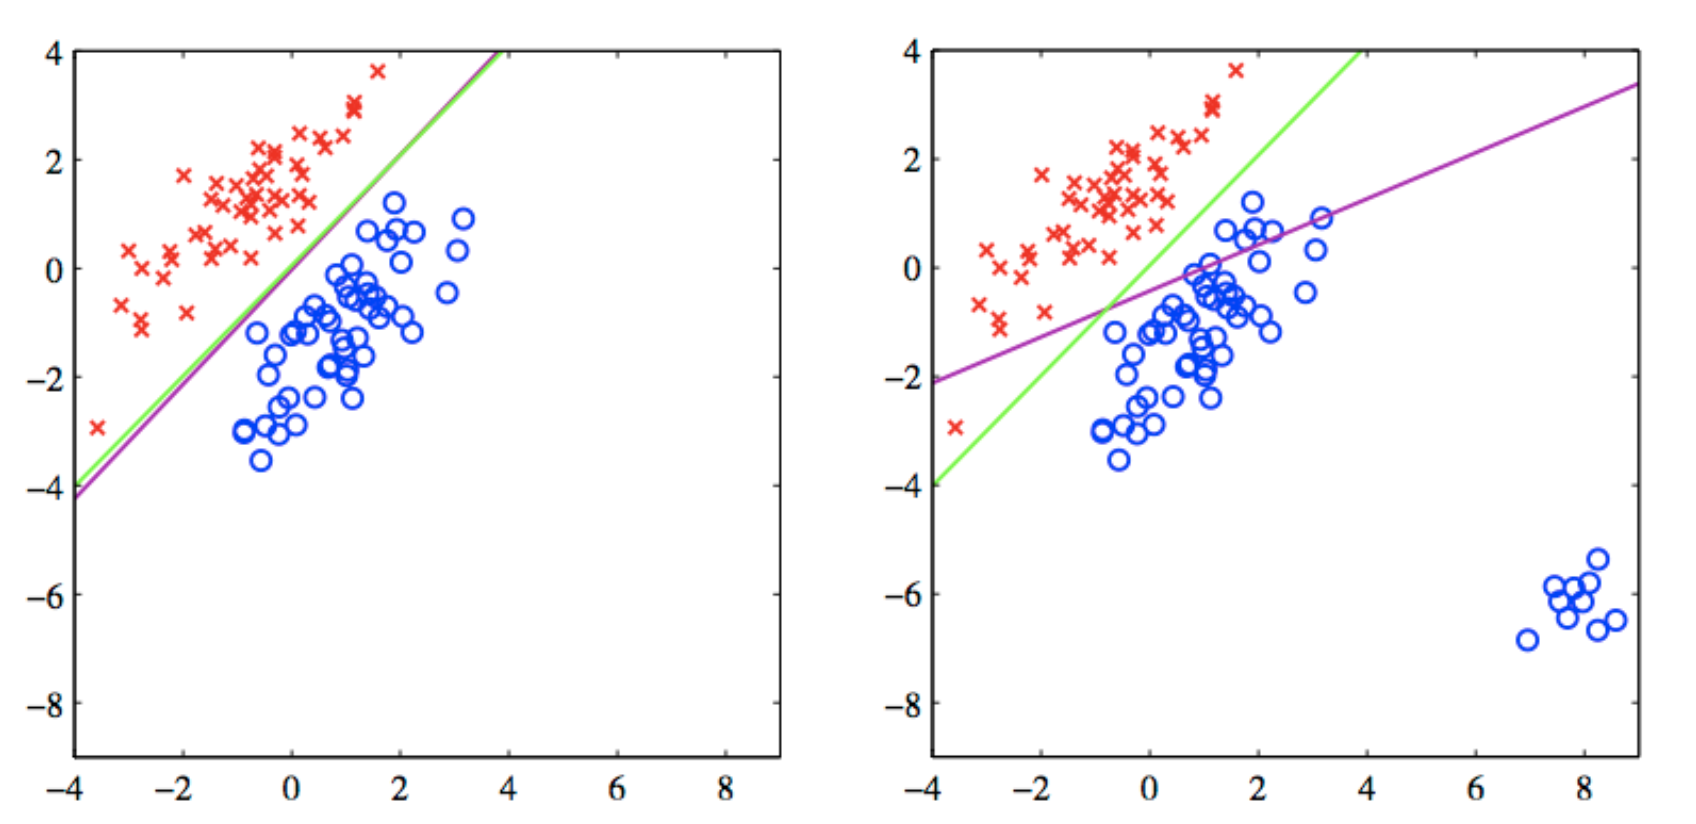
\includegraphics[width=300px, height=180px]{outlier_influence.png}
\end{center}
The two graphs show that the Logistic Regression Decision Boundary (the green line) is affected by outliers to a much lesser degree than the Linear Regression Decision Boundary (purple line).

\section{Bayesian Inference and Maximum Likelihood Estimation}

The goal of maximum likelihood estimation is to determine the most likely distribution from which a set of data is drawn. To do this, we begin by assuming the class of distributions from which the data is drawn and seek to find the most likely parameters of that distribution. Suppose the parameter for the distribution is $\beta$, where $\beta\sim\mathbb{P}(\beta)$. Note here that $\beta$ is a vector, where each component makes up a parameter of the sought after distribution. That is, given some set of data, every possible parameter of some distribution $\beta$ has some probability of being the true parameter of the distribution. We seek to find most likely distribution that the data came from. We draw labels according to the logistic model given by $\beta$. We begin by defining the function 
\begin{align*}
lik(\beta)=\prod_{i=1}^{n} \mathbb{P}(X_i,Y_i \mid \beta)
\end{align*}

which defines the probability of observing the data given a certain parameter $\beta$. 

Using Bayes' Theorem, we can say that 
\begin{align*}
\mathbb{P}(\beta\mid X_1,Y_1,X_2,Y_2,\ldots,X_n,Y_n)=\frac{\mathbb{P}(X_1,Y_1,X_2,Y_2,\ldots,X_n,Y_n\mid\beta)\mathbb{P}(\beta)}{\mathbb{P}(X_1,Y_1,X_2,Y_2,\ldots,X_n,Y_n)}=\frac{lik(\beta)\mathbb{P}(\beta)}{\mathbb{P}(X_1,Y_1,X_2,Y_2,\ldots,X_n,Y_n)}.
\end{align*}

The most likely $\beta$ given the data $X_1,Y_1,X_2,Y_2,\ldots,X_n,Y_n$ therefore maximizes $lik(\beta)\mathbb{P}(\beta)$. Because $log(x)$ is a convex function, the maximum of $lik(\beta)\mathbb{P}(\beta)$ occurs at the same $\beta$ value as the maximum of $log(lik(\beta)\mathbb{P}(\beta)$). Using properties of logarithms, we seek to maximize 
\begin{align*}
log(lik(\beta)+log(\mathbb{P}(\beta)).
\end{align*}
\section{Multinomial Logistic Regression}
Multinomial logistic regression enables classification of objects into one of more than just two categories. Consider a random variable $Y$, which can be classified into $m$ categories. We write this as $Y\in \{1,\ldots,m\}$. Now, we posit the distribution 
\begin{align*}
\mathbb{P}(Y=j \mid X=x)\hskip 5pt \propto\hskip 5pt e^{\beta^T_jx}. 
\end{align*}

In order for this to be a valid probability distribution, we must ensure that
\begin{align*}
\sum_{j=1}^{m} \mathbb{P}(Y=j \mid X=x)=1.
\end{align*}
We can re-express this as 
\begin{align*}
\mathbb{P}(Y=j \mid  X=x)=\frac{e^{\beta^T_jx}}{\sum_{j=1}^{m}e^{\beta^T_jx}}. 
\end{align*}

If we fix $\beta_m=\vec{0}$, we can fit models by multinomial logistic regression using maximum likelihood estimation for the other components of $\beta$. 

\title{}
\section{Computing Logistic Regression}
Recall:
\begin{equation*}
L(\beta)=\sum_{i=1}^{n} (\log(1+e^{\beta^T x_i})-Y_i \beta^T X_i)
\end{equation*}
Since $L(\beta)$ is a convex function, we can expect its minimum occurs at critical points.\\
\\
So it is equal to solving:
\begin{equation*}
\bigtriangledown_\beta L(\beta)=
\begin{pmatrix}
\alpha L(\beta)/\alpha \beta_1\\
...\\
...\\
...\\
\alpha L(\beta)/\alpha \beta_p\\
\end{pmatrix}
=
\sum_{i=1}^{n}(\dfrac{e^{\beta^T x_i} x_i}{1+e^{\beta^T x_i}}-Y_i X_i)
=
\sum_{i=1}^{n} (\sigma (\beta^T x_i)-Y_i)X_i
=
\vec{0}
\end{equation*}
Which is a system of p equations in p unknowns.
We want to pick $\hat{\beta}$ that solves the above equation.\\
\\Recall for all i, we have $x_{i1}$=1. That implies:\\
\begin{equation*}
\sum_{i=1}^{n}(\sigma (\beta^T x_i)-Y_i))=0
\end{equation*}
Which is equivalent to:
\begin{equation*}
\dfrac{1}{n}\sum_{i=1}^{n}\sigma (\beta^T x_i)=\dfrac{1}{n}\sum_{i=1}^{n}Y_i
\end{equation*}
The left hand side of the above equation is the expected fraction of positive examples given logistic regression model with $\hat{\beta}$. And the right hand side is equal to the fraction of positive examples in the training data.

\section{The Newton-Raphson Method}
Logistic regression models are usually fit by maximum likelihood. We will make use of its derivatives to maximize the log likelihood $\ell(\beta)$. This sets the stage for this optimization problem and brings us to a classic problem: root-finding, and a classic algorithm: Newton's method (also known as the Newton–Raphson method, named after Isaac Newton and Joseph Raphson).

Logistic regression models are usually fit by maximum likelihood. As described at the end of last lecture, we will make use of its derivatives to maximize the log likelihood $\ell(\beta)$. This sets the stage for this optimization problem and brings us to a classic problem: root-finding, and a classic algorithm: Newton's method (also known as the Newton–Raphson method, named after Isaac Newton and Joseph Raphson). 

Fig.\ \ref{fig:newton} is an example of Newton's method from Wikipedia. To find the root of a function (shown in blue), we start with an initial guess $x_1$ and fit a tangent line using its first derivative if it exists. The tangent line is an approximation of the function at that point. Then we get new point $x_2$, which is assumed to be the root. Because the function is complex and we can see it is off the correct root. Then we use $x_2$ as the next guess. We repeat the process until a sufficiently accurate value is reached. Note that this is only guaranteed to provide us a local optimum.

Fig.\ \ref{fig:newton2} shows an instance of a Newton-type methods that uses both the first and second derivatives for a 1D function to find a local maximum of function $f(x)$. We start with a guess at $x_k$. Instead of fitting a tangent line to the function to generate the next guess, we fit a local quadratic approximation, i.e., a function that has the same 1st and 2nd derivatives as the target function. We can easily solve for the maximum of this new function and obtain the next guess for the maximum, $x_k+d_k$. We repeat this process until convergence.

\subsection{Solving LR with Newton-Raphson}
In our case we wish to solve the related problem of finding the maximum of a function. We will do this using both the first and second derivatives. In higher dimensions, as with our log likelihood $\mathcal{L}(\beta)$ where $\beta\in\mathbb{R}^{p+1}$, the counterparts to the 1st and 2nd derivatives are the gradient and the Hessian, respectively.
 

\begin{equation}
\mathcal{L}(\beta) = \sum_{i=1}^n \left \{ log(1+ e^{\beta ^\top x_i})  -  y_i \beta ^\top x_i \right \}
\label{eqn:llgrad}
	\end{equation}
    
\begin{figure}
\centering
\subfigure[Start with a guess $x_1$, find the tangent line using the first derivative, extrapolate to get next guess $x_2$.]{
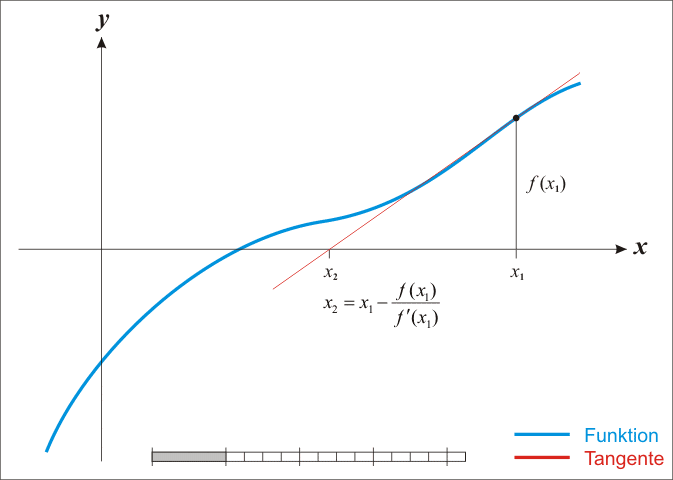
\includegraphics[width=0.45\textwidth]{NewtonIteration_Ani1.png}}
\quad
\subfigure[Repeat this process to get $x_3$, which as we can see overshoots in this case.]{
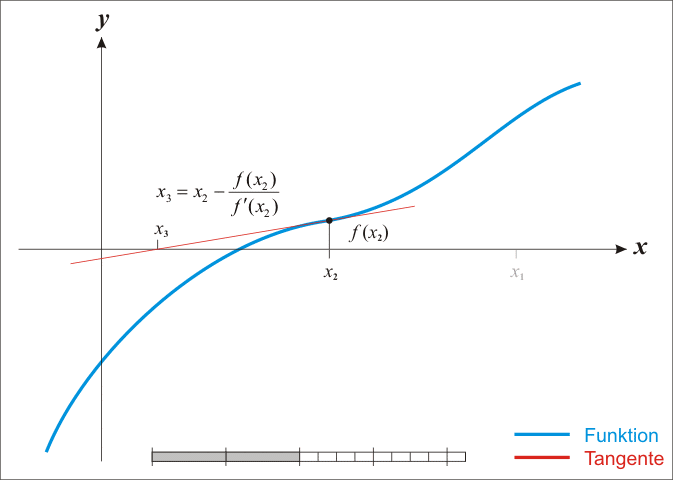
\includegraphics[width=0.45\textwidth]{NewtonIteration_Ani2.png}}

\subfigure[Keep iterating]{
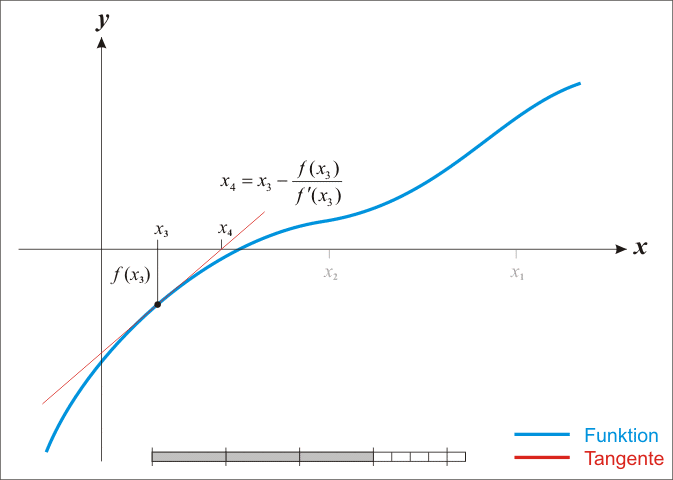
\includegraphics[width=0.45\textwidth]{NewtonIteration_Ani3.png}}
\quad
\subfigure[until a sufficiently accurate value is reached.]{
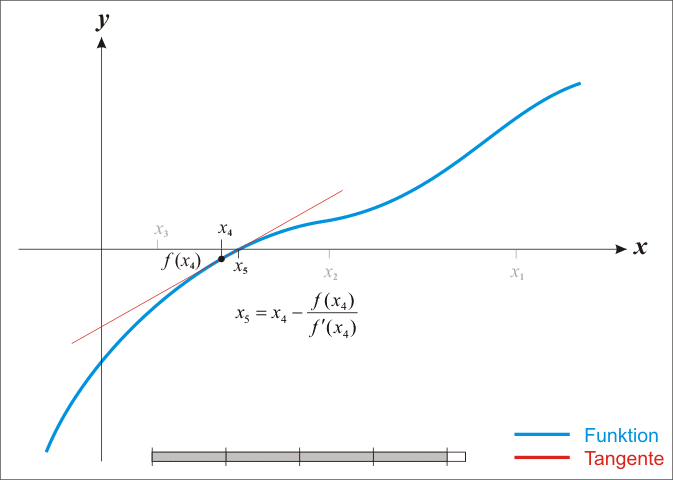
\includegraphics[width=0.45\textwidth]{NewtonIteration_Ani4.png}}
\caption{Illustration of Newton's method for finding a root. (Wikipedia)}
\label{fig:newton}
\end{figure}


\begin{figure}
\centering
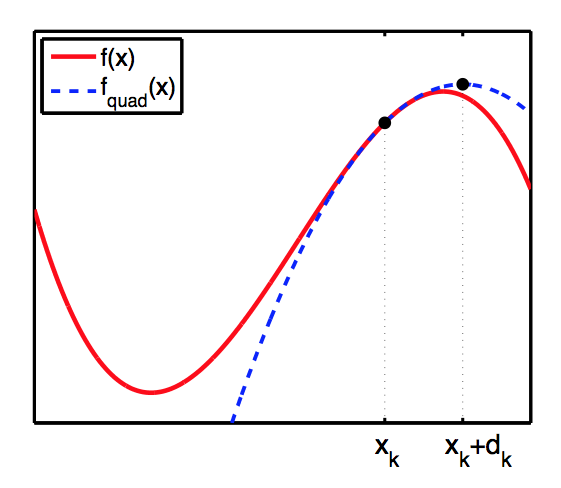
\includegraphics[width=0.6\textwidth]{newton_noncvx.png}
\caption{Finding a local maximum of a function $f(x)$ using a quadratic approximation.  We start with a guess at $x_k$.  Using both the 1st and 2nd order derivatives we fit a quadratic approximation to the function at that point.  That function $f_{\text{quad}}(x)$, is equivalent to the 2nd order Taylor series approximation of $f(x)$ around $x_k$.  We can easily solve for the maximum of this function and obtain the next guess for the maximum, $x_k+d_k$. We repeat this process until convergence. (Murphy)}
\label{fig:newton2}
\end{figure}


The gradient of the log likelihood is given by
\begin{equation}
\nabla_\beta\mathcal{L}(\beta) = \sum_{i=1}^{n}(\sigma (\beta^T x_i)-Y_i))
\label{eqn:llgrad}
	\end{equation}
Note that the gradient is a length $p+1$ vector.  We can see from this expression that the gradient can be expressed as a sum of feature vectors $x_i\in\mathbb{R}^{p+1}$, $i=1,\ldots,n$, weighted by $\sigma (\beta^T x_i)-Y_i$.

The Hessian of $\mathcal{L}(\beta)$, which is a $(p+1)\times(p+1)$ matrix, is given by
$$
\nabla_\beta^2 \mathcal{L}(\beta) = \sum_{i=1}^n \sigma (\beta^T x_i)\left(1-\sigma (\beta^T x_i)\right)x_i x_i^\top
$$
This matrix is a sum of terms of the form $x_i x_i^\top$ weighted by $\sigma (\beta^T x_i)\left(1-\sigma (\beta^T x_i)\right)$ and it characterizes the curvature of the function we're trying to minimize. Each $x_i x_i^\top$ term is the \textit{outer product} of $x_i$ with itself, resulting in a symmetric matrix of size $(p+1)\times(p+1)$.  We will see soon that this is closely related to how we compute the \emph{covariance matrix} for $\left\{x_i\right\}_1^n$. The scalar weight $\sigma (\beta^T x_i)\left(1-\sigma (\beta^T x_i)\right)$ has a small value when $\sigma(\beta^T x_i)$ is close to $y_i$. If $\sigma (\beta^T x_i)$ is close to $1$ then $1-\sigma (\beta^T x_i)$ is close to $0$ and vice versa, which means that if the approximation is good at least one multiplier in the expression $\sigma (\beta^T x_i)\left(1-\sigma (\beta^T x_i)\right)$ is close to $0$. As a result, the entire expression has a very low value far from the decision boundary. If $\sigma (\beta^T x_i)$ is a bad approximation of $y_i$ there is a higher chance that the classification is incorrect and as such $\sigma (\beta^T x_i)$ is closer to $0.5$, $1 - \sigma (\beta^T x_i)$ is also close to $0.5$ making the entire expression close to its maximum: $0.25$. If we look back at the Hessian we can now see that the sum emphasizes $x_i$s for which we are less certain of their classification making the contribution to the Hessian  larger when the choice of $\beta$ results in a poor decision boundary. 

\begin{figure}
\centering
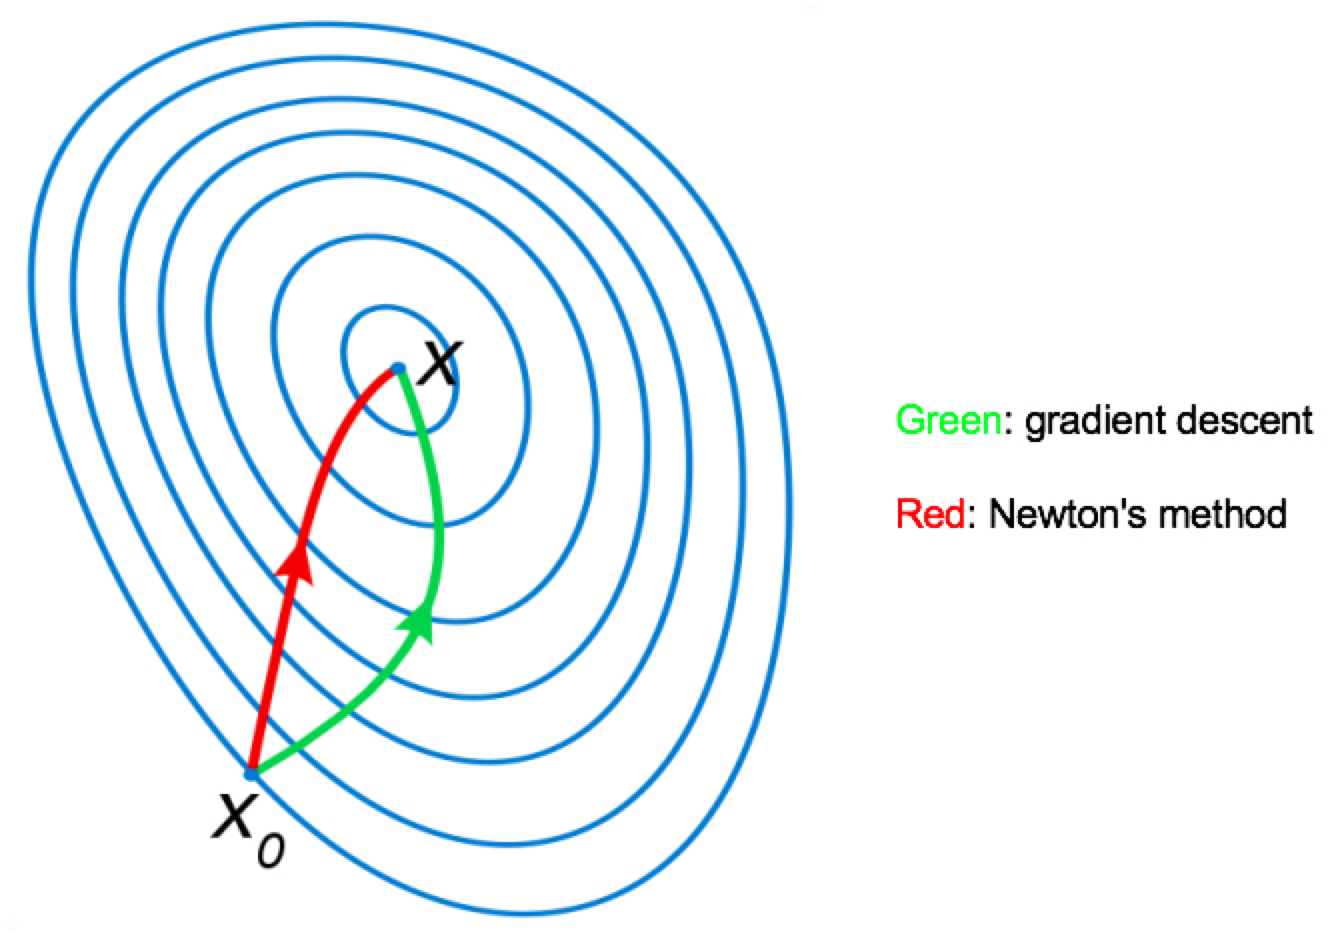
\includegraphics[width=1\textwidth]{Newton_s_Optimization.jpg}
\caption{A comparison of gradient descent (green) and Newton's method (red) for minimizing a function (with small step sizes). Newton's method uses curvature information to take a more direct route. (Wikipedia)}
\label{fig:newton3}
\end{figure}


Fig.\ \ref{fig:newton3} is a comparison of gradient descent (green) and Newton's method (red) for minimizing a function with small step sizes (the name of method varies depending on the reference) but the green curve is a classic first-order method and the red curve uses first- and second-order information. The first-order tells you something about the slope, and it will eventually get you to the local optimum by taking step in the direction of gradient. But if you take the curvature into account, which is indicated by the second-order derivative, you can get a more direct route. 


\subsection{Iterative Reweighted Least Squares (IRLS)}
In IRLS we start by picking a random choice for $\beta$ and apply a ``Newton update'' to get a better $\beta$. We continue taking Newton steps until we reach convergence. 
A Newton update is:
$$\beta^{new} = \beta^{old} - (\nabla_\beta^2 \mathcal{L}(\beta^{old}))^{-1}\nabla_\beta\mathcal{L}(\beta^{old})$$
in which the derivatives are evaluated at $\beta=\beta^{old}$.  If we put this in matrix notation we get:
$$\nabla_\beta\mathcal{L}(\beta) = \mathbf{X}^\top(\mathbf{y}-\mathbf{p})$$
$$\nabla_\beta^2 \mathcal{L}(\beta) = \mathbf{X}^\top \mathbf{W}\mathbf{X}$$
Where:
\begin{itemize}
  \item $\mathbf{y}$ is a vector of all the $y_i$s.
  \item $\mathbf{X}\in\mathbb{R}^{N\times (p+1)}$ is the matrix of all the feature vectors $x_i$s.
  \item $\mathbf{p}$ is a vector of the $\sigma (\beta^T x_i)s$.
  \item $\mathbf{W}\in\mathbb{R}^{N\times N}$ is a diagonal weighting matrix containing the values of $p_i(1 - p_i)   p_n(1-p_n)$ on the diagonal.
\end{itemize}
When we write the Newton update using this notation we get:
$$\beta^{new} = \beta^{old}+(\mathbf{X}^\top \mathbf{W}\mathbf{X})^{-1}\mathbf{X}^\top(\mathbf{y}-\mathbf{p})$$
$$\Downarrow$$
\begin{center}{(Multiply $\beta^{old}$ by $(\mathbf{X}^\top \mathbf{W}\mathbf{X})^{-1}(\mathbf{X}^\top \mathbf{W}\mathbf{X})$ which is the same as not changing it)}\end{center}
$$\beta^{new} = (\mathbf{X}^\top \mathbf{W}\mathbf{X})^{-1}(\mathbf{X}^\top \mathbf{W}\mathbf{X})\beta^{old}+(\mathbf{X}^\top \mathbf{W}\mathbf{X})^{-1}\mathbf{X}^\top(\mathbf{y}-\mathbf{p})$$
$$\Downarrow$$
\begin{center}(Factor out $(\mathbf{X}^\top \mathbf{W}\mathbf{X})^{-1}\mathbf{X}^\top \mathbf{W}$)\end{center}
$$\beta^{new} = (\mathbf{X}^\top \mathbf{W}\mathbf{X})^{-1}\mathbf{X}^\top \mathbf{W}(\mathbf{X}\beta^{old}+\mathbf{W}^{-1}(\mathbf{y}-\mathbf{p}))$$
$$\Downarrow$$
$$\beta^{new} = (\mathbf{X}^\top \mathbf{W}\mathbf{X})^{-1}\mathbf{X}^\top \mathbf{W}\mathbf{z}$$
in which $\mathbf{z}=\mathbf{X}\beta^{old}+\mathbf{W}^{-1}(\mathbf{y}-\mathbf{p})$. What is $\mathbf{z}$? We want to predict log odds but $\text{logit}(y_i) = \pm\infty$. Instead $\text{logit} \approx \text{logit}(\mathbf{p}) + (y-\mathbf{p})(\text{logit}'(\mathbf{p}))$ where $\mathbf{p} = \sigma(\beta^\top \mathbf{X})$.  We call $\mathbf{z}$ the \textit{adjusted response}.\\
In every IRLS iteration we solve this equation with a new set of $\mathbf{p}$, $\mathbf{W}$ and $\mathbf{z}$. This iteration solves the following weighted least squares problem over and over:
$$\beta^{new}\leftarrow\underset{\beta}{\arg\min}\sum_{i=1}^{n}\mathbf{W}_i(\beta^\top\mathbf{X}_i - \mathbf{z}_i)^2$$
(Recall $W$ is diagonal.)
We iterate this step until  convergence. 
This is named \emph{Iteratively Reweighted Least Squares} since in every iteration it solves a weighted least squares problem.

One remaining question is, how do we initialize $\beta$? Starting with $\beta=0$ is often OK.  Another option is to use multiple randomized restarts to reduce the chances of getting stuck at a local maximum.

\begin{figure}
\centering
\subfigure{
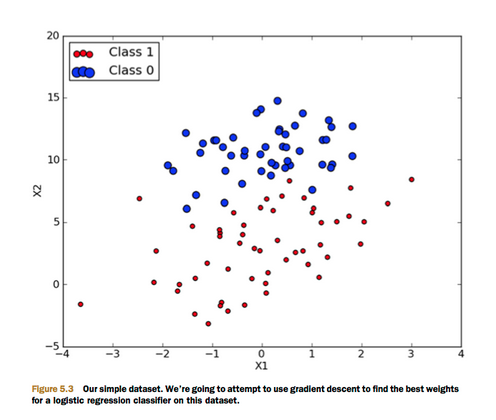
\includegraphics[width=0.45\textwidth]{HarringtonExample1.png}}
\quad
\subfigure{
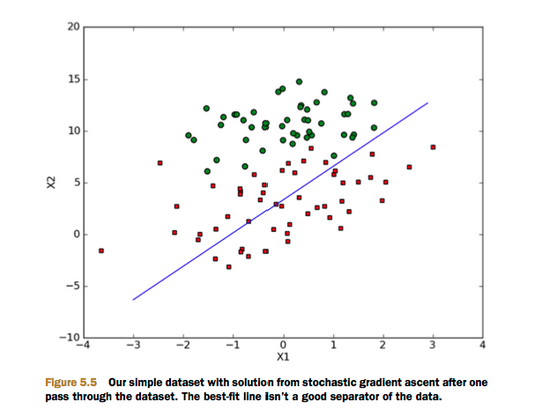
\includegraphics[width=0.45\textwidth]{HarringtonExample2.png}}

\subfigure{
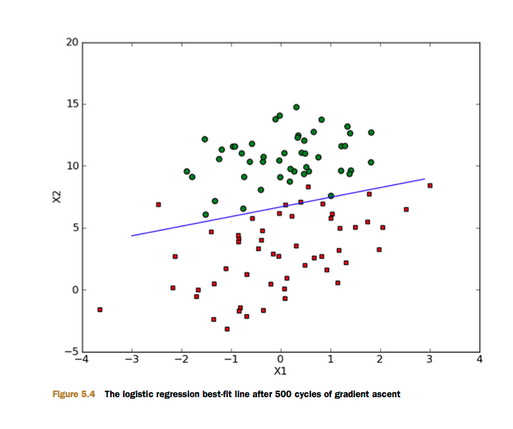
\includegraphics[width=0.45\textwidth]{HarringtonExample3.png}}
\quad
\caption{Logistic regression example (Harrington)}
\label{fig:Harrington}
\end{figure}





\end{document}
